\chapter{Evaluation} \label{chp:Evaluation}
In this chapter we want to present and discuss our evaluation results. Using Baselines Lab, we perform tests in a variety of different scenarios. After explaining our general test procedure in Section \ref{sec:TestProcedure}, we will begin, by evaluating the basic components for solving maze environments. In Section \ref{sec:EvalReward} we will take a look at reward generation and continue with a deeper look into observation generation and preprocessing in Section \ref{sec:EvalObs}. Section \ref{sec:EvalRLAlgorithms} will shine some light on the question which learning algorithm performs best when dealing with our particle navigation task and we will wrap up the evaluation of the basic parameters in Section \ref{sec:EvalParameters} where we take a look at the influence of various RL hyperparameters.

The initial tests will allow us to generate a baseline for the performance of our model, which then will be used throughout the rest of the evaluation to compare the influence of other factors. We begin, by testing how much inaccuracy in both actions and observations will influence the agent in Section \ref{sec:EvalError} and continue with the extension of the particle model with physical particles in Section \ref{sec:EvalPhysical}. We will then take a look at randomized instances in Section \ref{sec:EvalRandomness} and finish with a comparison with algorithmic approaches in Section \ref{sec:EvalAlgorithms}.


\section{Test Procedure} \label{sec:TestProcedure}
In this section we want to talk about different aspects of our test procedure.

\paragraph{Environment.}
All experiments were done on a Linux workstation running Ubuntu 18.04 LTS. The workstation has an Intel 6700K CPU, a single Nvidia GeForce GTX 1080 Ti GPU and 64GB of main memory. We installed Python 3.7.3 using the Anaconda \cite{anaconda} software distribution. We also used Tensorflow 1.14 in conjunction with the CUDA Toolkit version 10.1.243 and CUDNN version 7.6.5. Baselines Lab was developed on top of Stable-Baselines 2.10 and NumPy 1.17. For a complete list of installed packages see Appendix \ref{apx:BaselinesLab}.

\paragraph{Procedure.}
Our experiments involved several sources of randomness. To ensure consistent executions, we fixed the random seed for all involved components to the same value for all experiments. Unfortunately Tensorflow 1.14 does not guarantee consistent results during GPU computations. We therefore repeated experiments three times and averaged the results for comparison. The learning curves provided in this chapter are also smoothed by an exponential weighted moving average, using a factor of $0.6$.

To determine the performance of a configuration, we look at the end result during training for the average and best trial. We also determine the step in which the average episode length becomes smaller by five percent in comparison to the environments' time limit. We call this moment the \textit{drop}, since performance usually suddenly increases when the agent is able to reach the goal for the first time. The drop can be used as an indicator for how fast the agent is able to find a first usable result, while the end-of-training episode length is an indicator for how good the best solution is the agent is able to find. 

\paragraph{Initial Hyperparameters.}
For our initial experiments we wanted to use general purpose hyperparameters for the PPO algorithm. We therefore used parameters similar to the parameters used in the RND paper \cite{burda2018exploration} (see Table \ref{tab:RNDParameters}) which showed to produce good results across all Atari environments. 


\begin{table} [ht]
    \begin{center}
        \begin{tabular}{|c|c|}
            \hline
            Hyperparameter & Value \\
            \hline
            Rollout Length & 256 \\
            Number of minibatches & 8 \\
            Number of optimization epochs & 16 \\
            Number of parallel environments & 64 \\
            Learning rate & 0.0001 \\
            Optimization algorithm & Adam \cite{kingma2014adam} \\
            $\lambda$ & 0.95 \\
            Entropy coefficient & 0.001 \\
            $\gamma$ & 0.99 \\
            Clip range & [0.9, 1.1] \\
            \hline
        \end{tabular}
    \end{center}
    \caption[Default Hyperparameters]{Default hyperparameters for PPO for the initial experiments.} \label{tab:RNDParameters}
\end{table}

We also used a common preprocessing pipeline for the observations which was also used in previous experiments \cite{huang2019}:

\begin{table} [h]
    \begin{center}
        \begin{tabular}{|c|c|}
            \hline
            Hyperparameter & Value \\
            \hline
            Observation downsampling & (84, 84) \\
            Max steps per episode & 2000 \\
            Max and skip Frames & 4 \\
            Frame stacking & 4 \\
            \hline
        \end{tabular}
    \end{center}
    \caption[Default Observation Preprocessing]{Default observation preprocessing for all environments.} \label{tab:RNDParameters}
\end{table}

If not stated otherwise, we also normalized the observations by $x \mapsto x/255$. Observations for the RND curiosity module are normalized by $x \mapsto CLIP((x-\mu)/\sigma, [-5, 5])$ instead and no frame stacking is applied.


\paragraph{Instances.}
To allow easy comparison, we used the same instances as in previous work for our experiments. We included a description of these instances in Table \ref{tab:TestInstances}. Previous work showed, that these instances provide a good scale of difficulty between easy (\texttt{Corridor}) and hard (\texttt{Brain}). Instances with less paths to the goal position seem to be harder to solve, since they require more precise manoeuvering instead of just pulling all particles into a general direction. To increase the difficulty of our medium instance, we replaced it with an instance generated by our RRT instance generator. This instance can also be seen in Table \ref{tab:TestInstances} and is called \texttt{Vessel}. The Vessel maze has similar dimensions in comparison with Corridor, but has far more fine grained structures where particles may get stuck. There is also only a single path to the goal position. Additionally the Vessel maze only has a small percentage of blocked pixels, allowing for a lot more possible states than Corridor. 

\begin{table} [h!]
    \begin{center}
        \begin{tabular}{cccccc}
            \toprule
            Instance & Name & Dimension & Size (\% of Area) & $d_{avg}$ & $d_{max}$ \\
            \midrule
            
            \parbox[c]{3.5cm}{
\includegraphics[clip, width=3.5cm]{figures/evaluation/procedure/corridor_upscaled.png}} & Corridor & $(100 \times 100)$ & $2869 \ (= 28.69\%)$ & 73.65 & 117 \\
            \addlinespace[0.05cm]
            \midrule
            
            \parbox[c]{3.5cm}{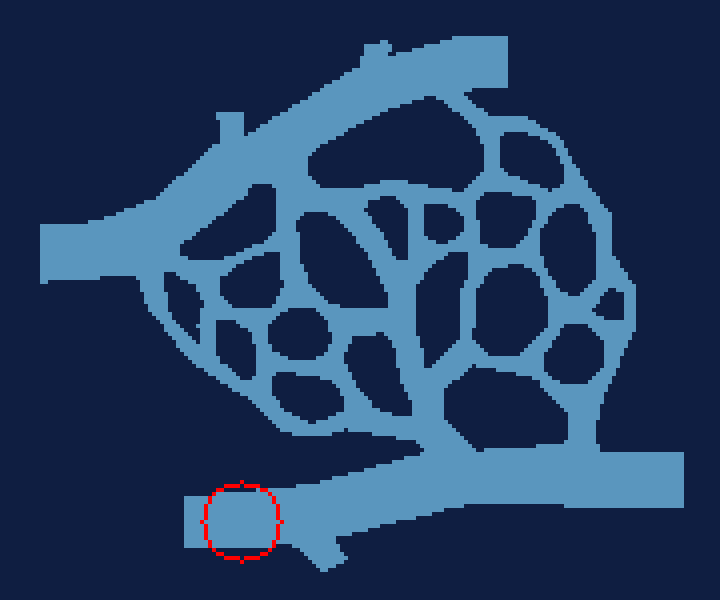
\includegraphics[clip, width=3.5cm]{figures/evaluation/procedure/capillary_upscaled.png}} & Capillary & $(180 \times 150)$ & $7169 \ (\approx 26.55\%)$ & 91.22 & 149 \\
            \addlinespace[0.05cm]
            \midrule
            
            \parbox[c]{3.5cm}{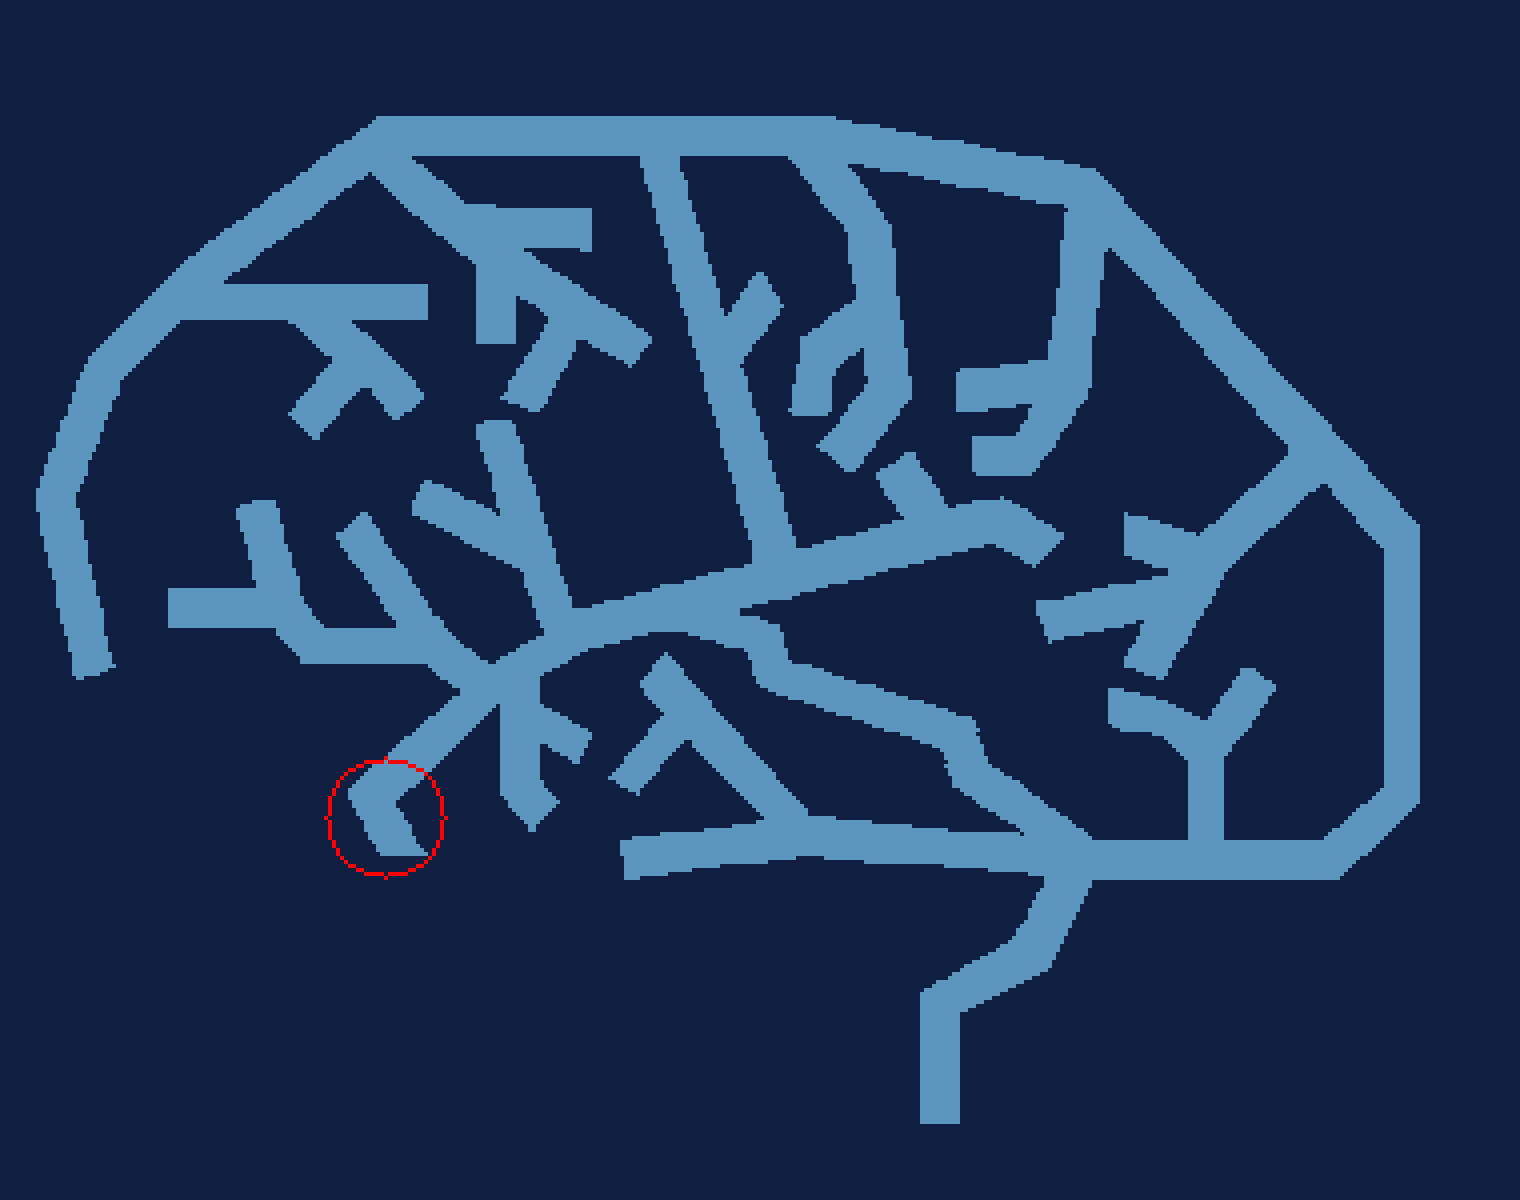
\includegraphics[clip, width=3.5cm]{figures/evaluation/procedure/brain_upscaled.png}} & Brain & $(380 \times 300)$ & $22593 \ (\approx 19.82\%)$ & 221.19 & 400 \\
            \addlinespace[0.05cm]
            \midrule
            
            \parbox[c]{3.5cm}{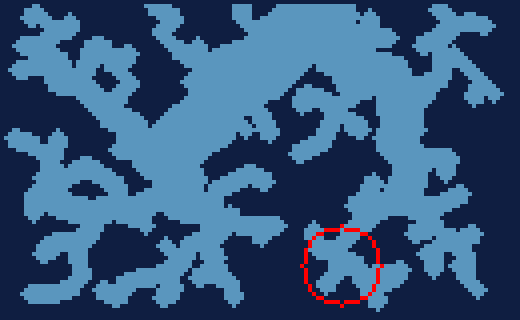
\includegraphics[clip, width=3.5cm]{figures/evaluation/procedure/vessel_upscaled.png}} & Vessel & $(130 \times 80)$ & $4949 \ (\approx 47.59\%)$ & 77.47 & 136 \\
            \addlinespace[0.05cm]
            \bottomrule
        \end{tabular}
    \end{center}
    \caption[Test Instances]{A list of our default test instances. Light blue pixels denote non-blocked pixels. The goal position is marked with a red circle. \textit{Dimension} describes the absolute size of the instance, while \textit{size} denotes the actual non-blocked area. We also included values for the average $d_{avg}$ and maximum $d_{max}$ distance between any point and the goal position.} \label{tab:TestInstances}
\end{table}

If not stated otherwise, we used 256 randomly generated particles for each episode during training. Episode lengths are capped at a maximum of 2000 steps independent of the environment. Dynamic episode lengths can also not exceed this hard cap.

\section{Reward Generation} \label{sec:EvalReward}
In this section we want to analyze how the reward generation influences training performance. In Section \ref{sec:RewardTestResults} we show our results and highlight key findings. We then continue to analyze some of the more important findings in Section \ref{sec:RewardAnalysis} and finish with our conclusion in Section \ref{sec:RewardConclusion}.

Since rewards are a key element to reinforcement learning, we expect that different rewards will heavily impact training performance. Our reward system provides a huge number of possible combinations of reward components and we therefore decide to use an iterative testing approach: We first test many combinations on the easy Corridor instance and then only evaluate the promising combinations on the Vessel instance. We finally select only the best performing combinations from the Vessel instance and test them on the Brain instance. Since observation normalization can have a huge impact on training performance and directly influences reward generation in the case of intrinsic reward, we also decided to add a second form of observation normalization in the form of $x \mapsto CLIP((x - \mu)/\sigma, [-10, 10])$ into this experiment. Note that the observation normalization of $x \mapsto x/255$ is always used if the second normalization option is not used.

Throughout this section we will provide a number of tables, which use abbreviations to save space. The abbreviations are explained in Table \ref{tab:RewardAbbreviations}.  

\begin{table} [ht]
    \begin{center}
        \small
        \begin{tabular}{ll}
            \toprule
            \multicolumn{1}{c}{Reward Component} & Abbreviation \\
            \midrule
            Continuous Reward & CR \\
            Discrete Reward & DR \\
            Observation Normalization & ON \\
            Reward Normalization & RN \\
            Time Penalty & TP \\
            Dynamic Episode Length & DEL \\
            Curiosity Reward & RND \\
            Gathering Reward & GR \\
            \bottomrule
        \end{tabular}
    \end{center}
    \caption[Abbreviations for Reward Components]{Common abbreviations for reward components} \label{tab:RewardAbbreviations}
\end{table}


\subsection{Test Results} \label{sec:RewardTestResults}

\paragraph{Corridor Environemnt.}
We begin with our easy instance Corridor. In our tests, we use the basic settings from Section \ref{sec:TestProcedure} and train for 3 million steps per trial. Table \ref{tab:Maze0318/Reward/Discrete} contains the results for discrete rewards and Table \ref{tab:Maze0318/Reward/Continuous} contains the results for continuous rewards.

Looking at the data, we can see, that many parameters do work very well and our dense discrete reward produces results which result in vastly shorter training times than in previous work \cite{huang2019}. Our initial experiments for discrete reward also show some interesting findings: 
\begin{itemize}
    \item \textbf{Normalization. } We found, that normalization has a huge impact on training performance. Normalizing the reward has a positive impact on its own (see Experiments 4/6), but additionally normalizing the observation by mean and standard deviation seems to be very important to improve performance in comparison to simple normalization (see Experiments 7/11 or 8/10).
    \item \textbf{Curiosity. } Using our relatively dense discrete reward, curiosity does not seem to have a positive effect for simple instances. Using DEL, a small amount of curiosity reward seems to have a positive impact (see Experiments 1/3), but also can have a negative impact if the weight is higher (see Experiments 1/2 or 13/14). Curiosity may have a greater impact when training with more complex instances though.
    \item \textbf{Dynamic Episode Length. } DEL does not seem to have any positive impact on the training performance. Experiment 9 shows that DEL is capable of creating time penalty like pressure, but the final result is worse than training with our normal time penalty. In combination with curiosity reward or a standard time penalty, performance seems to also worsen. (see Experiments 11/13; 12/14)
    \item \textbf{Gathering Reward. } Gathering reward does not seem to have any influence on the performance for small instances. Further testing will show, if this changes with larger or more challenging instances, where gathering of particles before bringing them to the goal might be more beneficial.
\end{itemize}


\begin{table}[htp]
    \begin{center}
        \begin{tabular}{rccccccrrr}
            \toprule
             & \multicolumn{6}{c}{Reward Component} & \multicolumn{2}{c}{Episode Length} & \\
            \cmidrule(lr){2-7}\cmidrule(lr){8-9}
            \multicolumn{1}{c}{Idx} & \multicolumn{1}{c}{ON} & \multicolumn{1}{c}{RN} & \multicolumn{1}{c}{TP} & \multicolumn{1}{c}{DEL} & \multicolumn{1}{c}{RND} & \multicolumn{1}{c}{GR} & \multicolumn{1}{c}{Best} & \multicolumn{1}{c}{Avg} & \multicolumn{1}{c}{Drop}\\
            \midrule
            1 &  &  &  & X &  &  & 256.78 & 295.04 & 1.25M \\
            2 &  &  &  & X & 0.50 &  & 499.97 & 499.99 & 750k \\
            3 &  &  &  & X & 0.25 &  & 110.94 & 117.82 & 750k \\
            4 &  &  & X &  &  &  & 135.03 & 145.34 & 629k \\
            5 &  &  & X &  & 0.25 &  & 324.29 & 422.48 & 456k \\
            6 &  &  & X & X &  &  & 477.62 & 491.48 & 3M \\
            7 &  & X & X &  &  &  & 83.78 & 84.66 & 461k \\
            8 &  & X & X &  &  & 1.00 & 93.31 & 94.30 & 406k \\
            9 & X & X &  & X &  &  & 65.72 & 67.17 & 400k \\
            10 & X & X & X &  &  & 1.00 & 59.31 & \textbf{65.68} & 190k \\
            11 & X & X & X &  &  &  & \textbf{57.38} & 66.81 & 182k \\
            12 & X & X & X &  & 0.50 &  & 84.52 & 207.78 & \textbf{181k} \\
            13 & X & X & X & X &  &  & 65.34 & 78.93 & 400k \\
            14 & X & X & X & X & 0.50 &  & 500.00 & 500.00 & 3M \\
            \bottomrule
        \end{tabular}
    \end{center}
    \caption[Evaluation of Discrete Reward Evaluation with the Corridor Environment]{Evaluation of discrete rewards with the corridor environment.} \label{tab:Maze0318/Reward/Discrete}
\end{table}


The evaluation results using continuous reward show similar outcomes to the experiments using discrete reward. The most important finding is, that the best continuous reward is able to produce superior results in every category compared to the best discrete reward. Especially the time of first notable improvement is about 30\% earlier. We included a plot showing the average episode length during training in Figure \ref{fig:ContinuousVsDiscrete}. This further supports our decision to create more dense rewards. 

\begin{table}[htp]
    \begin{center}
        \begin{tabular}{rccccccccrrr}
            \toprule
             & \multicolumn{8}{c}{Reward Component} & \multicolumn{2}{c}{Episode Length} & \\
            \cmidrule(lr){2-9}\cmidrule(lr){10-11}
            \multicolumn{1}{c}{Idx} & \multicolumn{1}{c}{ON} & \multicolumn{1}{c}{RN} & \multicolumn{1}{c}{TP} & \multicolumn{1}{c}{DEL} & \multicolumn{1}{c}{RND} & \multicolumn{1}{c}{GR} & \multicolumn{1}{c}{Int Norm} & \multicolumn{1}{c}{PO} & \multicolumn{1}{c}{Best} & \multicolumn{1}{c}{Avg} & \multicolumn{1}{c}{Drop}\\
            \midrule
            1 &  &  &  & X &  &  & X &  & 101.06 & 106.07 & 600k \\
            2 &  &  &  & X & 0.25 &  & X &  & 394.12 & 413.82 & 800k \\
            3 &  &  & X &  &  &  &  &  & 146.38 & 149.47 & 787k \\
            4 &  &  & X &  &  &  & X &  & 102.44 & 103.96 & 718k \\
            5 &  &  & X & X &  &  & X &  & 92.12 & 96.00 & 400k \\
            6 &  & X & X &  &  &  & X & X & 90.47 & 98.18 & 370k \\
            7 &  & X & X &  &  &  & X &  & 101.62 & 102.40 & 525k \\
            8 &  & X & X &  &  & 1.00 & X &  & 96.22 & 103.99 & 614k \\
            9 &  & X & X &  & 0.25 &  & X &  & 198.44 & 335.29 & 561k \\
            10 & X & X &  & X &  &  & X &  & 82.41 & 83.32 & 400k \\
            11 & X & X & X &  &  &  &  &  & \textbf{56.59} & \textbf{59.04} & \textbf{127k} \\
            12 & X & X & X &  &  &  & X & X & 58.72 & 65.46 & 152k \\
            13 & X & X & X &  &  &  & X &  & 61.81 & 71.28 & 147k \\
            14 & X & X & X &  &  & 1.00 &  &  & 60.53 & 62.46 & 149k \\
            15 & X & X & X &  &  & 1.00 & X &  & 59.09 & 68.69 & 151k \\
            16 & X & X & X &  & 0.25 &  & X & X & 69.41 & 246.38 & 158k \\
            17 & X & X & X & X &  &  & X & X & 79.19 & 79.39 & 400k \\
            \bottomrule
        \end{tabular}
    \end{center}
    \caption[Evaluation of Continuous Reward with the Corridor Environment]{Evaluation of continuous rewards with the corridor environment.} \label{tab:Maze0318/Reward/Continuous}
\end{table}


\begin{figure}[htp]
    
    \begin{center}
        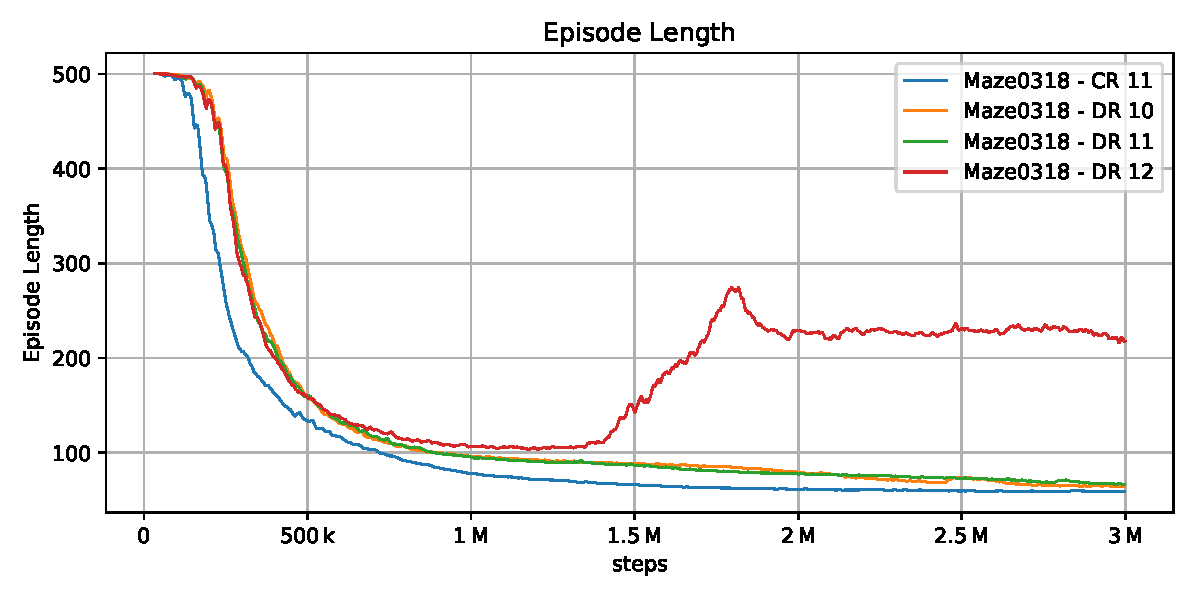
\includegraphics[clip, width=0.75\columnwidth]{figures/evaluation/rewards/continuous_vs_discrete.pdf}
    \end{center}
    
    %\vspace*{-6pt}
    \caption[Training Curves with Curiosity Reward]{Average episode length on the corridor environment during training. The legend refers to experiment numbers.}
    \label{fig:ContinuousVsDiscrete}
    %\vspace*{-12pt}
\end{figure}

\begin{figure}[htp]
    
    \begin{center}
        \begin{tabular}{c}
            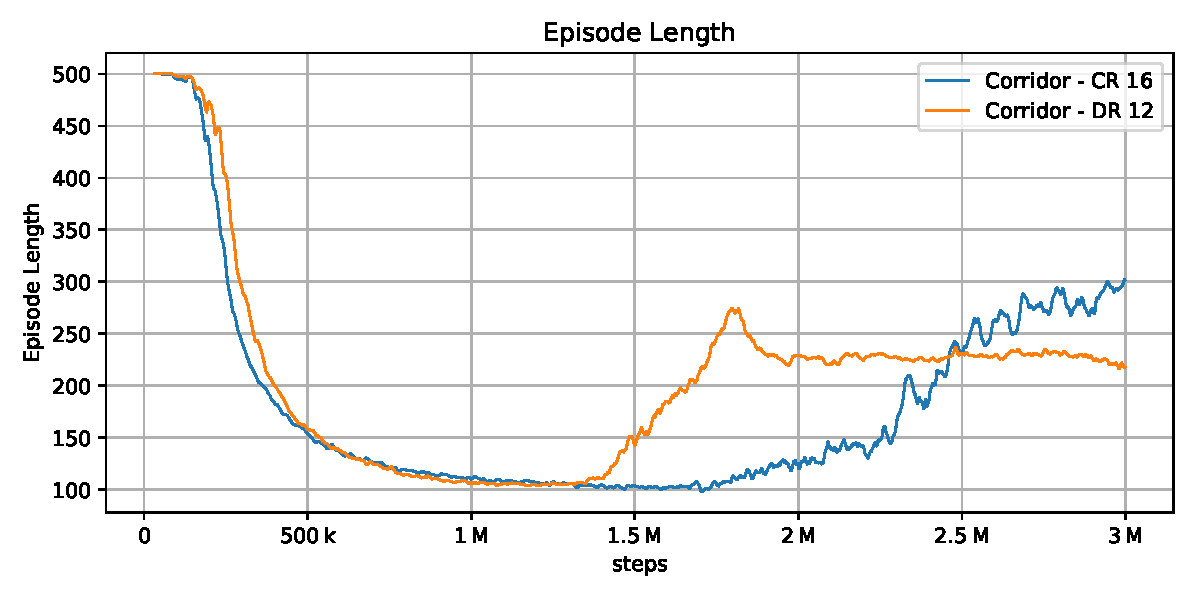
\includegraphics[clip, width=0.75\columnwidth]{figures/evaluation/rewards/curiosity_divergence_ep_len.pdf} \\
            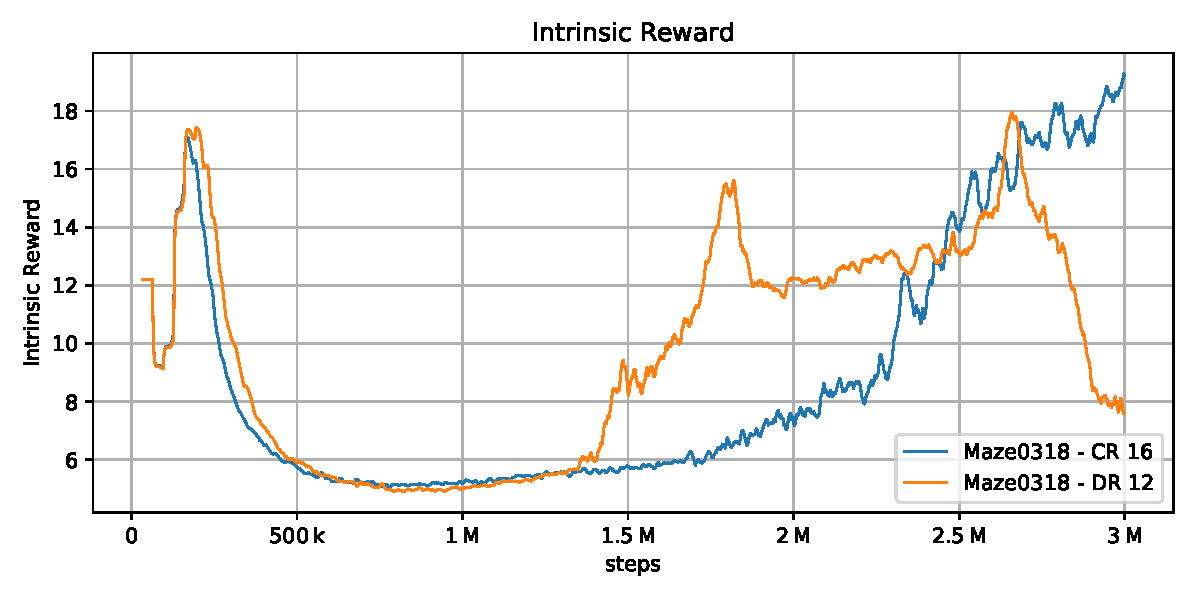
\includegraphics[clip, width=0.75\columnwidth]{figures/evaluation/rewards/curiosity_divergence_int_rew.pdf} \\
            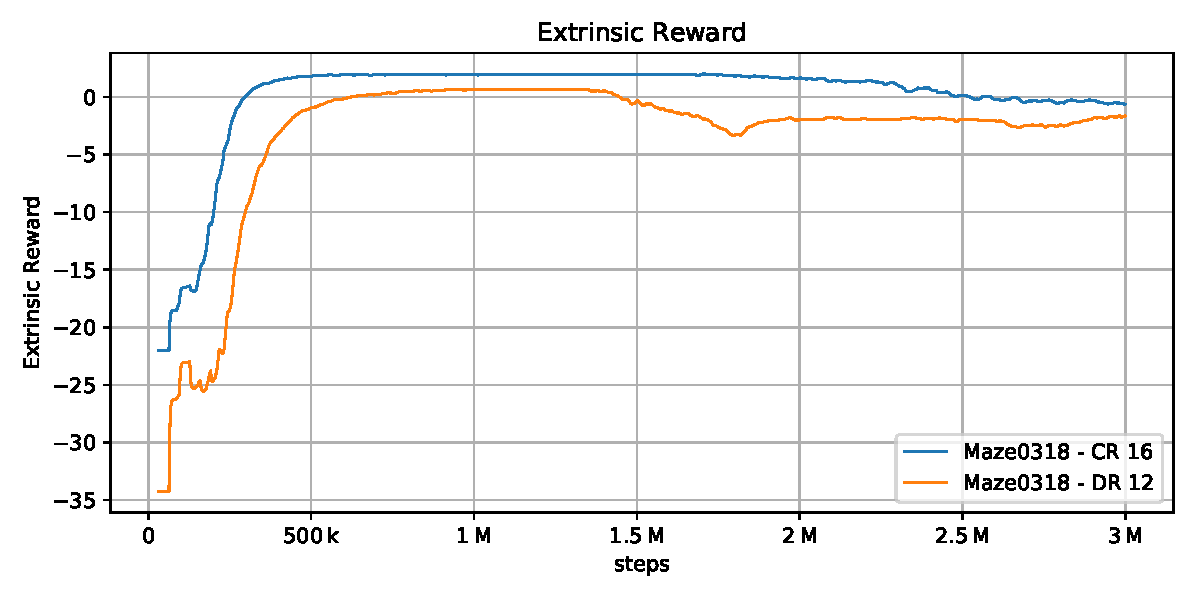
\includegraphics[clip, width=0.75\columnwidth]{figures/evaluation/rewards/curiosity_divergence_ext_rew.pdf}
        \end{tabular}

    \end{center}
    
    %\vspace*{-6pt}
    \caption[Problems with Curiosity Reward]{Learning curves for training with curiosity reward. We observed, that intrinsic rewards increase the chance for a performance collapse during training in terms of episode length. This can be seen, by comparing the intrinsic to the extrinsic reward and looking at the episode length at the same time: At around 1.5 million training steps, the intrinsic reward begins to increase, while the extrinsic reward remains at a constant level. At the same time, the average episode length begins to increase.}
    \label{fig:CuriosityDiverge}
    %\vspace*{-12pt}
\end{figure}


Similar to the results obtained when using discrete rewards, we can see, that observation normalization by mean and standard deviation massively improves performance for continuous rewards. Curiosity also does not seem to improve the results and often tends to diverge from the optimum at the end of training as shown in Figure \ref{fig:CuriosityDiverge}. Otherwise the corridor instance seems to be too easy to show differences between other reward parameters. Like before, gathering reward does not seem to have any positive or negative impact. The use of positive only rewards shows to improve performance without normalization (see Experiments 3/4), but only has a small impact with normalization (see Experiments 12/13). Interestingly internal normalization which balances the total cost reward against the maximum cost reward has shown to worsen the results on the corridor environment (see Experiments 11/13). 


\paragraph{Vessel Environment.} We repeat multiple experiments on the more complicated, but similarly large vessel instance. The results for discrete rewards are shown in Table \ref{tab:VesselMaze02/Reward/Discrete} and the results for continuous reward in Table \ref{tab:VesselMaze02/Reward/Continuous}. To compensate for the more complex environment, we double the training time for the agent and train for 6 millions steps per trial. 

Looking at the results for discrete rewards in Table \ref{tab:VesselMaze02/Reward/Discrete}, we can see, that normalization is crucial for success. While agents trained with non-normalized rewards are still able to find solutions, they need much more training time. For discrete rewards, the addition of a supporting reward signals seems to be important: The experiments including dynamic episode length (3), gathering reward (5) or curiosity reward (6) all produced better results, than stand-alone discrete reward (4). Especially the combination of discrete reward with curiosity was able to find a solution in a relatively short time. Note, that training with curiosity is significantly slower due to the extra computation for the training of the predictor network. 

\begin{table}[htp]
    \begin{center}
        \begin{tabular}{rccccccrrr}
            \toprule
             & \multicolumn{6}{c}{Reward Component} & \multicolumn{2}{c}{Episode Length} & \\
            \cmidrule(lr){2-7}\cmidrule(lr){8-9}
            \multicolumn{1}{c}{Idx} & \multicolumn{1}{c}{ON} & \multicolumn{1}{c}{RN} & \multicolumn{1}{c}{TP} & \multicolumn{1}{c}{DEL} & \multicolumn{1}{c}{RND} & \multicolumn{1}{c}{GR} & \multicolumn{1}{c}{Best} & \multicolumn{1}{c}{Avg} & \multicolumn{1}{c}{Drop}\\
            \midrule
            1 &  &  &  & X & 0.25 &  & 478.91 & 487.95 & 9.99M \\
            2 &  &  & X &  & 0.25 &  & 491.19 & 497.06 & 9.99M \\
            3 & X & X &  & X &  &  & \textbf{89.38} & 95.75 & 1.2M \\
            4 & X & X & X &  &  &  & 97.28 & 100.09 & 762k \\
            5 & X & X & X &  &  & 1.00 & 93.78 & \textbf{95.15} & 828k \\
            6 & X & X & X &  & 0.50 &  & 107.31 & 109.18 & \textbf{694k} \\
            7 & X & X & X & X &  &  & 89.62 & 96.38 & 1.2M \\
            \bottomrule
        \end{tabular}
    \end{center}
    \caption[Evaluation of Discrete Reward Evaluation with the Vessel Environment]{Evaluation of discrete rewards with the vessel environment.} \label{tab:VesselMaze02/Reward/Discrete}
\end{table}


The results for continuous rewards differ from the results for discrete rewards. By looking at Table \ref{tab:VesselMaze02/Reward/Continuous} we can see, that the addition of supporting rewards often produces worse results (see Experiments 7/11, 4/5, 8/10). An exception seems to be the combination of gathering reward with not internally normalized reward (see Experiments 6/9). Using only positive reward, does not seem to improve performance. The same is true for dynamic episode lengths.  


\begin{table}[htp]
    \begin{center}
        \begin{tabular}{rccccccccrrr}
            \toprule
             & \multicolumn{8}{c}{Reward Component} & \multicolumn{2}{c}{Episode Length} & \\
            \cmidrule(lr){2-9}\cmidrule(lr){10-11}
            \multicolumn{1}{c}{Idx} & \multicolumn{1}{c}{ON} & \multicolumn{1}{c}{RN} & \multicolumn{1}{c}{TP} & \multicolumn{1}{c}{DEL} & \multicolumn{1}{c}{RND} & \multicolumn{1}{c}{GR} & \multicolumn{1}{c}{Int Norm} & \multicolumn{1}{c}{PO} & \multicolumn{1}{c}{Best} & \multicolumn{1}{c}{Avg} & \multicolumn{1}{c}{Drop}\\
            \midrule
            1 &  &  & X &  & 0.25 &  & X &  & 451.00 & 476.26 & 7.92M \\
            2 &  & X & X &  &  &  &  &  & 423.09 & 433.16 & 7.81M \\
            3 &  & X & X &  &  &  & X & X & 373.28 & 405.12 & 8M \\
            4 &  & X & X &  &  &  & X &  & 416.28 & 458.89 & 7.91M \\
            5 &  & X & X &  &  & 1.00 & X &  & 418.75 & 470.94 & 7.05M \\
            6 & X & X & X &  &  &  &  &  & 93.97 & 98.73 & \textbf{501k} \\
            7 & X & X & X &  &  &  & X & X & 103.16 & 105.57 & 628k \\
            8 & X & X & X &  &  &  & X &  & 91.06 & \textbf{96.72} & 532k \\
            9 & X & X & X &  &  & 1.00 &  &  & \textbf{89.41} & 100.26 & 600k \\
            10 & X & X & X &  &  & 1.00 & X &  & 95.16 & 98.65 & 507k \\
            11 & X & X & X &  & 0.25 &  & X & X & 126.94 & 197.88 & 601k \\
            12 & X & X & X & X &  &  & X & X & 185.62 & 193.65 & 2.8M \\
            \bottomrule
        \end{tabular}
    \end{center}
    \caption[Evaluation of Continuous Reward with the Vessel Environment]{Evaluation of continuous rewards with the vessel environment.} \label{tab:VesselMaze02/Reward/Continuous}
\end{table}

\paragraph{Brain Environment.} We finally tested our the best performing reward configurations from the vessel environment on the brain environment. To compensate for the larger instance size and increased complexity, we again doubled training times, resulting in a total of 12 million training steps per trial. 

The results for discrete reward are listed in Table \ref{tab:Maze0122/Reward/Discrete}. Surprisingly, two of the three selected rewards did perform very poorly. Neither the configuration with dynamic episode length nor the one with curiosity reward did yield acceptable end results after 12 million training steps. The only discrete reward variation that can solve the brain environment successfully under the given time limit uses additional gathering reward. 


\begin{table}[htp]
    \begin{center}
        \begin{tabular}{rccccccrrr}
            \toprule
             & \multicolumn{6}{c}{Reward Component} & \multicolumn{2}{c}{Episode Length} & \\
            \cmidrule(lr){2-7}\cmidrule(lr){8-9}
            \multicolumn{1}{c}{Idx} & \multicolumn{1}{c}{ON} & \multicolumn{1}{c}{RN} & \multicolumn{1}{c}{TP} & \multicolumn{1}{c}{DEL} & \multicolumn{1}{c}{RND} & \multicolumn{1}{c}{GR} & \multicolumn{1}{c}{Best} & \multicolumn{1}{c}{Avg} & \multicolumn{1}{c}{Drop}\\
            \midrule
            1 & X & X &  & X &  &  & 500.00 & 500.00 & 12M \\
            2 & X & X & X &  &  & 1.00 & \textbf{311.44} & \textbf{319.23} & \textbf{7.15M} \\
            3 & X & X & X &  & 0.50 &  & 479.59 & 486.36 & 12M \\
            \bottomrule
        \end{tabular}
    \end{center}
    \caption[Evaluation of Discrete Reward with the Brain Environment]{Evaluation of discrete rewards with the brain environment.} \label{tab:Maze0122/Reward/Discrete}
\end{table}

In contrast to the discrete reward variations, all continuous reward configurations were able to solve the brain environment. As we can see from Table \ref{tab:Maze0122/Reward/Continuous}, the addition of gathering reward yields the best results, while internally normalized (balanced) continuous reward performs better than non-balanced reward.

\begin{table}[htp]
    \begin{center}
        \begin{tabular}{rccccccccrrr}
            \toprule
             & \multicolumn{8}{c}{Reward Component} & \multicolumn{2}{c}{Episode Length} & \\
            \cmidrule(lr){2-9}\cmidrule(lr){10-11}
            \multicolumn{1}{c}{Idx} & \multicolumn{1}{c}{ON} & \multicolumn{1}{c}{RN} & \multicolumn{1}{c}{TP} & \multicolumn{1}{c}{DEL} & \multicolumn{1}{c}{RND} & \multicolumn{1}{c}{GR} & \multicolumn{1}{c}{Int Norm} & \multicolumn{1}{c}{PO} & \multicolumn{1}{c}{Best} & \multicolumn{1}{c}{Avg} & \multicolumn{1}{c}{Drop}\\
            \midrule
            1 & X & X & X &  &  &  &  &  & 328.97 & 352.97 & 7.46M \\
            2 & X & X & X &  &  &  & X &  & \textbf{308.31} & 333.53 & 7.34M \\
            3 & X & X & X &  &  & 1.00 & X &  & 324.78 & \textbf{333.35} & \textbf{6.75M} \\
            \bottomrule
        \end{tabular}
    \end{center}
    \caption[Evaluation of Continuous Reward with the Brain Environment]{Evaluation of continuous rewards with the brain environment.} \label{tab:Maze0122/Reward/Continuous}
\end{table}


\subsection{Analysis} \label{sec:RewardAnalysis}
While it is easy to understand that dense rewards provide more information to the agent and thus produced superior results, other aspects are not as clear. In this section we want to analyze the learned behavior under different reward settings, to get a better understanding why certain configurations work better than others.

\paragraph{Curiosity.} Intrinsic reward has been the key to success for previous work, while our experiments showed a negative influence on training performance. To understand this, we analyzed how episodes are solved by agents trained with and without curiosity. In Figure \ref{fig:curiosity_ep_analysis} we show metrics taken at each step over the course of a single episode on the corridor environment. Both agents were trained using continuous reward, using the settings from Experiment 11 (without curiosity) and Experiment 16 (with curiosity) on the corridor environment. 

\begin{figure}[htp]
    \begin{center}
        \begin{tabular}{c}
            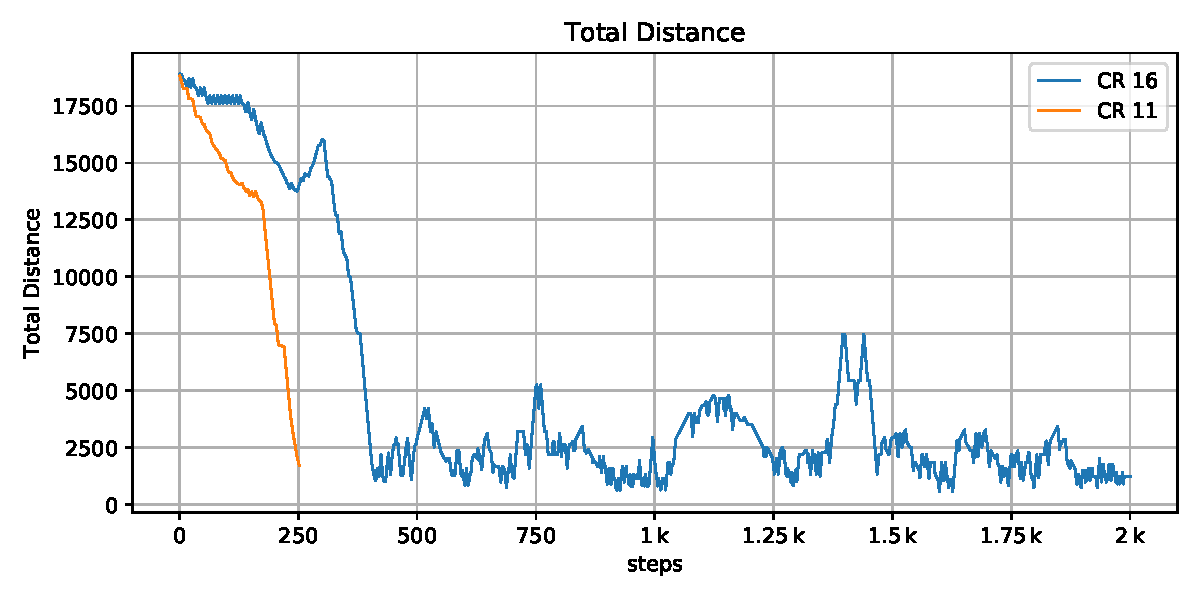
\includegraphics[clip, width=0.75\columnwidth]{figures/evaluation/rewards/episode_analysis/curiosity_total_distance.pdf} \\
            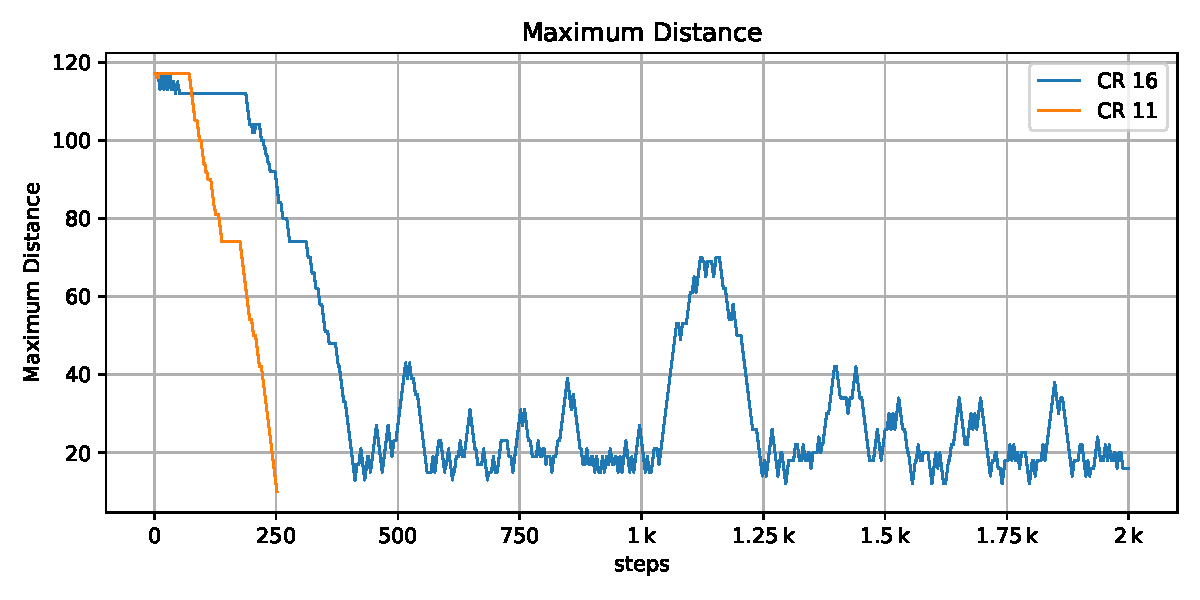
\includegraphics[clip, width=0.75\columnwidth]{figures/evaluation/rewards/episode_analysis/curiosity_max_distance.pdf} \\
            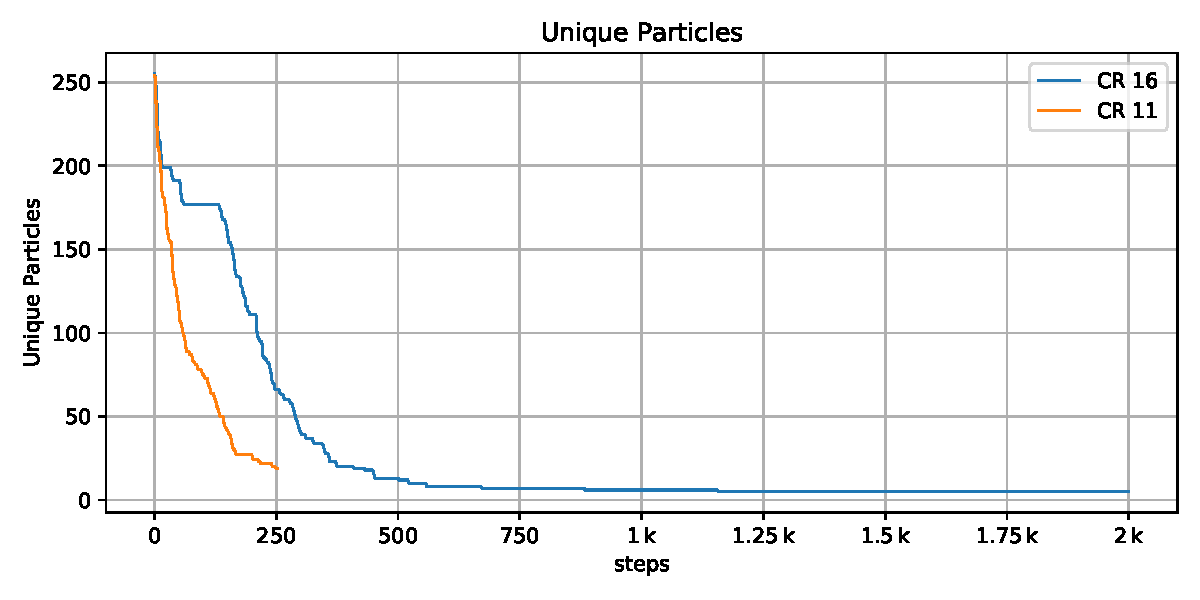
\includegraphics[clip, width=0.75\columnwidth]{figures/evaluation/rewards/episode_analysis/curiosity_unique_particles.pdf} \\
        \end{tabular}
    \end{center}
    \caption[Episode metrics on the Corridor Environment]{Metrics for a single example episode on the corridor instance. The steps are given without the MaxAndSkip wrapper and therefore in comparison 4 times larger. The blue line shows an agent trained with curiosity (see Experiment 16) and the orange line an agent trained without curiosity (see Experiment 11). The agent trained without curiosity is able to end the episode after about 250 steps, while the agent trained with curiosity does not end the episode during the 2000 steps time limit.} \label{fig:curiosity_ep_analysis}
\end{figure}


By looking at Figure \ref{fig:curiosity_ep_analysis} we can see, that both agents are able to reduce the total distance to the goal position very fast at the beginning of the episode. While the agent trained without curiosity finishes the episode after about 250 steps, the agent trained with curiosity decides to continue the episode by moving the particles back and forth close to the goal position. One could argue, that the agent might have to deal with a single particle that was left behind in the maze earlier, but this is not the case. We can see this by looking at the maximum distance any particle is away from the goal position. The particle which is the farthest away from the goal is closer than 20 pixels at around 470 steps and since the corridor environment only contains straight corridors, we can argue, that this particle cannot be stuck behind any obstacle. 

The question is why has the agent learned to not finish the episode when training with curiosity? We found, that there is a number of reasons why curiosity reward can be maximized by not finishing the episode. Let us begin with the easiest one: In Section \ref{sec:blRND} we showed, that an agent trained purely with curiosity learns to maximize episode lengths. Since it is able to explore more states during longer episodes, it can generate more intrinsic reward, if episodes are longer. The same happens in our particle environment where short episodes result in less intrinsic reward. Curiosity therefore works against our goal of achieving short episodes lengths. 

Another problem with curiosity comes from the nature of how the observations are generated in our environment: Since particles are directly shown in the observation and there are a lot of particles at the same time, the agent has control over a decent number of its own observation inputs. Since the agent is able to rapidly move the particles to appear at different positions, it is able to generate a massive amount of environment states and therefore observations similar to input noise. This situation is directly related to the \textit{noisy tv problem} described by Burda et al. \cite{burda2018large}. We can directly see this behavior in Figure \ref{fig:curiosity_ep_analysis}, where the agent has learned to increase the number of states, by gradually moving the particles to and away from the goal position, while slowly reducing the number of unique particles. Unfortunately this problem is not easy to fix. Implementing a large goal reward, may increase the number of episodes where the agent actually brings all particles to the goal, but the agent can still finish the episode at the last possible moment. Increasing the time penalty was found to help to some extend during our initial experiments. Previous experiments \cite{huang2019,becker2020} also used a larger time penalty and therefore may have not encountered this problem. Unfortunately we found that increasing the time penalty requires very careful fine-tuning for each environment to work correctly and therefore does not fix the underlying problem.

\paragraph{Strategies.}
One interesting aspect for the future choice of rewards would be, if the learned strategies differ depending on the given reward. Looking at the change of total distance to the goal position in the brain environment (see Figure \ref{fig:Rewards/Ep_Analysis}), we can assume, that the learned strategies are pretty similar. Except for agents trained with the discrete reward in combination with DEL or curiosity, the change in distances is very similar.  

\begin{figure}[htp]
    \begin{center}
        \begin{tabular}{c}
            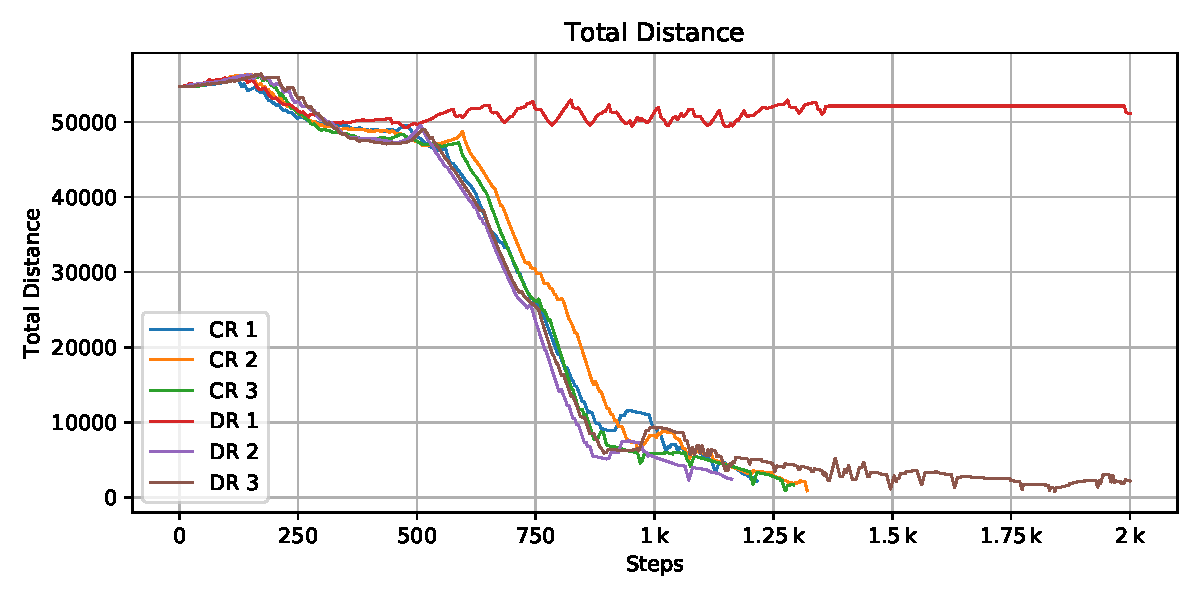
\includegraphics[clip, width=0.95\columnwidth]{figures/evaluation/rewards/episode_analysis/maze0122_total_dist.pdf} \\
            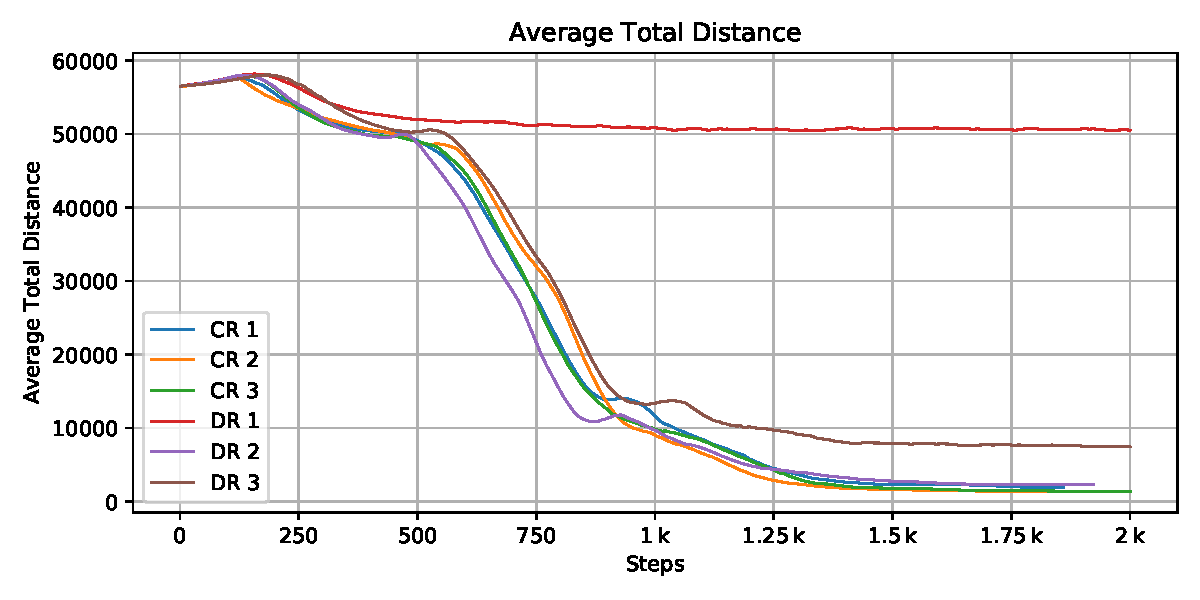
\includegraphics[clip, width=0.95\columnwidth]{figures/evaluation/rewards/episode_analysis/maze0122_total_dist_avg.pdf} \\
        \end{tabular}
    \end{center}
    \caption[Episode metrics on the Brain Environment]{Total sum of distances to the goal position over a single episode on the brain environment. On the top, we included a plot showing a single episode and on the bottom we included the average over 64 episodes.} \label{fig:Rewards/Ep_Analysis}
\end{figure}

To verify this result we monitor the similarity between actions for a given observation. We generate trajectories by replaying the different agents on the brain environment. We then replay the observations to all agents and count the differences in the choice of the best action (using stochastic policies). Note that an alternative measure would be to calculate an approximate Kullback-Leibler distance using the generated trajectories, but we found, that results are hard to interpret.

\begin{table}[htp]
    \begin{center}
        \begin{threeparttable}
            \begin{tabular}{l|rrrrrrr}
                \toprule
                vs & DR 2 & DR 2\tnote{1} & DR 3 & DR 1 & CR 2 & CR 3 & CR 1 \\
                \midrule
                DR 2 & 100.00 & 50.09 & 37.25 & 15.19 & 42.31 & 44.79 & 42.31 \\
                DR 2\tnote{1} & 50.09 & 100.00 & 45.41 & 10.89 & 39.33 & 43.84 & 45.83 \\
                DR 3 & 37.25 & 45.41 & 100.00 & 13.12 & 34.69 & 36.73 & 39.75 \\
                DR 1 & 15.19 & 10.89 & 13.12 & 100.00 & 15.68 & 18.43 & 15.10 \\
                CR 2 & 42.31 & 39.33 & 34.69 & 15.68 & 100.00 & 45.19 & 50.73 \\
                CR 3 & 44.79 & 43.84 & 36.73 & 18.43 & 45.19 & 100.00 & 48.54 \\
                CR 1 & 42.31 & 45.83 & 39.75 & 15.10 & 50.73 & 48.54 & 100.00 \\
                \bottomrule
            \end{tabular}
            \begin{tablenotes} \footnotesize
                \item[1] This agent uses the same reward as DR2, but from a different trial.
            \end{tablenotes}
        \end{threeparttable}
    \end{center}
    \caption[Agent Action Similarity for Different Rewards]{Similarity of actions between different agents given in percent of equal actions for the same observation on the brain environment. Similarity is measured by first generating observations by replaying the agents and then comparing the actions different agents would have chosen in the same situation.} \label{tab:Maze0122/Reward/Similarity}
\end{table}

We included the results in terms of percent of equal actions for the same observations in Table \ref{tab:Maze0122/Reward/Similarity}. A surprising result is, that two agents trained with the \textit{same} reward only produce the same action for about 50\% of the observations. The most reasonable explanation is that we have a set with very similar actions (e.g. NE, N, NW) and there are many situations where either of these actions can be used. Different neural networks then evolved into using only one of them for a specific input and therefore produce very dissimilar results for the same observation, even when trained with the same reward. Keeping this baseline in mind, we can see, that agents trained with different rewards also differ in their percentage of equal actions. Most notably the both worst performing agents trained with discrete reward (DR 1 and DR 3). For all other agents, the differences are significantly smaller. We can therefore assume, that the learned strategies only differ slightly and the agents all evolved into learning an similar optimized strategy independent of the used reward. 

\subsection{Conclusion} \label{sec:RewardConclusion}
When deciding for a reward for our further experiments, we have to keep in mind, that every extra computation will be executed for each individual training step. The more reward components we use, the longer training will take. When comparing the results on the brain environment for continuous reward, we saw that the addition of gathering reward just slightly improves the average end result. If we look at the wall-clock time, trials using the gathering reward took an average of 4:51h to complete, while trials using only the continuous reward took 4:22h on average. This means that with gathering reward, we saw an increase of about 11\% more time. While additional components might provide benefits for special environments (see Section \ref{sec:EvalRandomness}) they do not provide significant improvements for our general case. Depending on the environment size, multiple rewards can be used to achieve good performance, but only a few scale well into larger instances. We therefore will use continuous internally normalized reward for all further experiments.

\section{RL Algorithms} \label{sec:EvalRLAlgorithms}
RL Algorithms, Hyperparameter optimization, etc

\paragraph{Result Variation}
Variation

\section{Observations} \label{sec:EvalObs}
\begin{table}[htp]
    \begin{center}
        \begin{tabular}{rcrrrr}
            \toprule
            \multicolumn{1}{c}{Idx} & \multicolumn{1}{c}{Frame Size} & \multicolumn{1}{c}{Best} & \multicolumn{1}{c}{Avg} & \multicolumn{1}{c}{Drop} & \multicolumn{1}{c}{Time}\\
            \midrule
            1 & (168, 168) & 356.47 & 356.47 & \textbf{6.22M} & 17:49:36h \\
            2 & (84, 84) & \textbf{308.31} & \textbf{333.53} & 7.34M & 4:28:39h \\
            3 & (44, 44) & 500.00 & 500.00 & 12M & 3:06:27h \\
            4 & (24, 24) & 500.00 & 500.00 & 12M & \textbf{2:54:06h} \\
            \bottomrule
        \end{tabular}
    \end{center}
    \caption{Maze0122}
\end{table}

\begin{table}[htp]
    \begin{center}
        \begin{tabular}{rcrrrr}
            \toprule
            \multicolumn{1}{c}{Idx} & \multicolumn{1}{c}{Frame Size} & \multicolumn{1}{c}{Best} & \multicolumn{1}{c}{Avg} & \multicolumn{1}{c}{Drop} & \multicolumn{1}{c}{Time}\\
            \midrule
            1 & (100, 100) & \textbf{60.75} & \textbf{65.57} & 157k & 1:00:46h \\
            2 & (84, 84) & 61.81 & 71.28 & \textbf{147k} & 0:40:36h \\
            3 & (44, 44) & 78.00 & 79.42 & 181k & 0:21:17h \\
            4 & (24, 24) & 82.28 & 84.67 & 209k & 0:22:12h \\
            5 & (12, 12) & 500.00 & 500.00 & 1.41M & \textbf{0:15:19h} \\
            \bottomrule
        \end{tabular}
    \end{center}
    \caption{Maze0318}
\end{table}

\begin{table}[htp]
    \begin{center}
        \begin{tabular}{rcrrrr}
            \toprule
            \multicolumn{1}{c}{Idx} & \multicolumn{1}{c}{Frame Size} & \multicolumn{1}{c}{Best} & \multicolumn{1}{c}{Avg} & \multicolumn{1}{c}{Drop} & \multicolumn{1}{c}{Time}\\
            \midrule
            1 & (130, 80) & 98.38 & 100.20 & 539k & 2:03:17h \\
            2 & (84, 84) & \textbf{91.06} & \textbf{96.72} & 532k & 1:10:00h \\
            3 & (44, 44) & 105.03 & 112.49 & 566k & 0:43:36h \\
            4 & (24, 24) & 99.38 & 107.81 & \textbf{501k} & 0:45:29h \\
            5 & (12, 12) & 494.75 & 495.42 & 6M & \textbf{0:31:24h} \\
            \bottomrule
        \end{tabular}
    \end{center}
    \caption{VesselMaze02}
\end{table}


\section{Extended Environment Models} \label{sec:EvalExtendedModels}
Extended Environment Models
\subsection{Dealing with Error} \label{sec:EvalError}
Dealing with Error
\subsection{Physical Particles} \label{sec:EvalPhysical}
Physical Particles
\section{Randomized Instances} \label{sec:EvalRandomness}
Randomized Instances
\subsection{Random Goal Positions} \label{sec:EvalRandomGoals}
Random Goal Positions
\subsection{Random Mazes} \label{sec:EvalRandomMaze}
Random Mazes
\section{Comparison to Algorithmic Approaches} \label{sec:EvalAlgorithms}
Comparison to Algorithmic Approaches